\documentclass[11pt]{article}
\usepackage{enumitem}
\usepackage{listings}
\usepackage[listings]{tcolorbox}
\usepackage{tikz}
\usepackage{url}
\usepackage{alltt}
\usepackage{amsfonts}
\usepackage{ebproof}

%\usepackage{algorithm2e}
\usetikzlibrary{arrows,automata,shapes}
\tikzstyle{block} = [rectangle, draw, fill=blue!20, 
    text width=5em, text centered, rounded corners, minimum height=2em]
\tikzstyle{bt} = [rectangle, draw, fill=blue!20, 
    text width=1em, text centered, rounded corners, minimum height=2em]

\lstset{ %
language=Java,
basicstyle=\ttfamily,commentstyle=\scriptsize\itshape,showstringspaces=false,breaklines=true,numbers=left}
\newtcbinputlisting{\codelisting}[3][]{
    extrude left by=1em,
    extrude right by=2em,
    listing file={#3},
    fonttitle=\bfseries,
    listing options={basicstyle=\ttfamily\footnotesize,numbers=left,language=Java,#1},
    listing only,
    hbox,
}
\lstdefinelanguage{JavaScript}{
  keywords={typeof, new, true, false, catch, function, return, null, catch, switch, var, if, in, while, 
do, else, case, break},
  keywordstyle=\color{blue}\bfseries,
  ndkeywords={class, export, boolean, throw, implements, import, this},
  ndkeywordstyle=\color{darkgray}\bfseries,
  identifierstyle=\color{black},
  sensitive=false,
  comment=[l]{//},
  morecomment=[s]{/*}{*/},
  commentstyle=\color{purple}\ttfamily,
  stringstyle=\color{red}\ttfamily,
  morestring=[b]',
  morestring=[b]''
}


\newtheorem{defn}{Definition}
\newtheorem{crit}{Criterion}

\newcommand{\handout}[5]{
  \noindent
  \begin{center}
  \framebox{
    \vbox{
      \hbox to 5.78in { {\bf Software Testing, Quality Assurance and Maintenance } \hfill #2 }
      \vspace{4mm}
      \hbox to 5.78in { {\Large \hfill #5  \hfill} }
      \vspace{2mm}
      \hbox to 5.78in { {\em #3 \hfill #4} }
    }
  }
  \end{center}
  \vspace*{4mm}
}

\newcommand{\lecture}[4]{\handout{#1}{#2}{#3}{#4}{Lecture #1}}
\topmargin 0pt
\advance \topmargin by -\headheight
\advance \topmargin by -\headsep
\textheight 8.9in
\oddsidemargin 0pt
\evensidemargin \oddsidemargin
\marginparwidth 0.5in
\textwidth 6.5in

\parindent 0in
\parskip 1.5ex
%\renewcommand{\baselinestretch}{1.25}

\begin{document}

\lecture{5 --- January 20, 2025}{Winter 2025}{Patrick Lam}{version 1}

The big topic for today is semantics. In SE 212 you saw axiomatic semantics,
which generally are used to prove program correctness. There are other ways of
reasoning about programs, though, namely operational semantics and denotational
semantics. In this coure we are going to use operational semantics, and it's going
to be needed for some of the reasoning that we're going to do.

\section*{Defining WHILE, a simple imperative language}
Languages are complicated. We're going to work on a language, which
we'll call WHILE\footnote{Sometimes a similar language is called IMP.}. We've
removed almost everything from it. And yet, it still shows the
essential complications of reasoning about code.  You had a similar
language in SE212.

Here's an example program.
\begin{lstlisting}
  { p := 0; x := 1; n := 2 };
  while x <= n do {
    x := x + 1;
    p := p + m
  } ; 
  print_state
\end{lstlisting}
Note that ; separates statements. Contrast this to C, where you end statements with a ;.

\paragraph{Syntactic entities.} The syntactic entities of WHILE are as follows. We first have terminals:
\begin{itemize}[noitemsep]
\item $n \in \mathbb{Z}$: integers;
\item $\textsf{true}, \textsf{false} \in B$: Booleans;
\item $x, y \in L$: locations (program variables);
\end{itemize}
as well as non-terminals:
\begin{itemize}[noitemsep]
\item $a \in \mathit{Aexp}$: arithmetic expressions;
\item $b \in \mathit{Bexp}$: Boolean expressions; and,
  \item $c \in \mathit{Stmt}$: statements.
\end{itemize}

Terminals are leaves in the Abstract Syntax Tree, and completely
defined by their tokens (rather than their relationships to other AST
nodes). Non-terminals contain zero or more terminals in terms of
parsing, and contain zero or more AST tokens, as determined by the
grammar. The containment relationship is represented by AST edges.

\paragraph{Arithmetic Expressions.} We can now give a grammar for arithmetic expressions
$\mathit{Aexp}$.
\begin{eqnarray*}
e & ::= & n \hspace*{3em} (\mbox{for $n \in \mathbb{Z}$}) \\
  & | & x  \hspace*{3em} (\mbox{for $x \in \mathbb{L}$}) \\
  & | & \texttt{-}e \\
  & | & e_1 \mathit{~aop~} e_2 \\
  & | & \texttt{(}e\texttt{)}\\[1em]
aop & ::= & \texttt{+} \ |\ \texttt{-} \ |\  \texttt{*}
\end{eqnarray*}
Some notes:
\begin{itemize}[noitemsep]
\item Like in Python, you don't have to declare variables before use.
\item All variables are integer-typed. We have Boolean expressions, but not Boolean variables.
\item Expressions have no side-effects---all effects are explicit.
\end{itemize}

\paragraph{Boolean Expressions.} Also for boolean expressions $\mathit{Bexp}$.
\begin{eqnarray*}
b & ::= & \textsf{true} \\
  & | & \textsf{false} \\
  & | & \texttt{not~} b \\
  & | & e_1 \mathit{~rop~} e_2  \hspace*{3em} (\mbox{for $e_1, e_2 \in \mathit{Aexp}$}) \\
  & | & b_1 \mathit{~bop~} b_2  \hspace*{3em} (\mbox{for $b_1, b_2 \in \mathit{Bexp}$}) \\
  & | & \texttt{(}b\texttt{)}\\[1em]
rop & ::= & \verb+<+ \ |\ \verb+<=+  \ |\ \verb+=+ \ |\ \verb+>=+  \ |\ \verb+>+ \\
bop & ::= & \texttt{and} \ | \ \texttt{or}
\end{eqnarray*}

\paragraph{Statements.} Finally, statements $s$.
\begin{eqnarray*}
s & ::= & \texttt{skip} \\
  & | & x \texttt{:=} e \\
  & | & \texttt{if} ~b~ \texttt{then} ~s~ [\texttt{else}~s] \\
  & | & \texttt{while} ~b~ \texttt{do} ~s \\
  & | & \texttt{\{}\mathit{~slist~}\texttt{\}}\\
  & | & \texttt{print\_state} \\
  & | & \texttt{assert}~b \ | \ \texttt{assume}~b \ | \ \texttt{havoc~} v_1, \ldots, v_N \\
\mathit{slist} &::=& s~ ( \texttt{;} s )^*\\
\mathit{prog} &::=& \mathit{slist}  
\end{eqnarray*}

More notes:
\begin{itemize}[noitemsep]
\item The semicolon \texttt{;} separates statements, rather than terminating them.
\item All side-effects in WHILE are caused by statements (not expressions).
\item We've dropped many features from WHILE (references, function calls, \ldots), but it's still fiendishly hard to analyze!
\end{itemize}

\section*{Abstract Syntax Trees \& Visitors}

We've seen this before in Lecture 3, but the AST abstractly represents the source code in tree form; each node represents some syntactic construct from the code, e.g. statements, expressions, variables, operators. It's abstract because it drops the tokens like \texttt{(} as well as, for most langages, whitespace and comments. Order of operations is encoded in the tree edges.

Here's an AST for \texttt{(x + 3) * (y-5)}.
\begin{center}
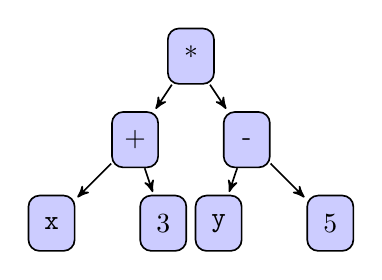
\begin{tikzpicture}[->,>=stealth',shorten >=1pt,auto,node distance=1.5cm,
                    semithick,initial text=]

  \node[bt]           (1) {*};
  \node[bt]           (2) [below left of=1, xshift=1em] {+};
  \node[bt]           (3) [below right of=1,xshift=-1em] {-};
  \node[bt]           (4) [below left of=2] {\tt x};
  \node[bt]           (5) [below right of=2,xshift=-2em] {3};
  \node[bt]           (6) [below left of=3,xshift=2em] {\tt y};
  \node[bt]           (7) [below right of=3] {5};

  \path (1) edge node {} (2)
  (1) edge node {} (3)
  (2) edge node {} (4)
  (2) edge node {} (5)
  (3) edge node {} (6)
  (3) edge node {} (7);
\end{tikzpicture}
\end{center}

The slides contain content about language parsing, but I'll assume you know this from CS 241.

\paragraph{WHILE AST implementation in Python.} Here is some code that implements a WHILE AST. It has
one class per syntactic entity, one field per child, and the class hierarchy corresponds to the
semantic hierarchy (i.e. the class encodes the type of node).

\begin{lstlisting}[language=Python]
class Ast(object):
  """Base class of AST hierarchy"""
  pass

class Stmt(Ast):
  """A single statement"""
  pass

class AsgnStmt(Stmt):
  """An assignment statement"""
  def __init__(self, lhs, rhs):
    self.lhs = lhs
    self.rhs = rhs

class IfStmt(Stmt):
  """If-then-else statement"""
  def __init__(self, cond, then_stmt, else_stmt=None):
    self.cond = cond
    self.then_stmt = then_stmt
    self.else_stmt = else_stmt
\end{lstlisting}

\paragraph{Visitor pattern.} I expect you to know about the visitor pattern from CS 247.
I'm just going to make two Python-specific comments:
\begin{itemize}[noitemsep]
\item instead of using polymorphism to visit, as done in Java, we find the target using the class name as part of the method, e.g. \texttt{visit\_Stmt()};
\item the \texttt{visit()} method of the Visitor uses reflection (it calls the method indicated by the string) rather than polymorphism to make the call, and hence we don't need \texttt{accept()}.
\end{itemize}

Here is an example Python visitor for WLANG:
\begin{lstlisting}[language=Python]
class AstVisitor(object):
    """Base class for AST visitor"""

    def __init__(self):
        pass

    def visit(self, node, *args, **kwargs):
        """Visit a node."""
        method = "visit_" + node.__class__.__name__
        visitor = getattr(self, method)
        return visitor(node, *args, **kwargs)

    def visit_BoolConst(self, node, *args, **kwargs):
        visitor = getattr(self, "visit_" + Const.__name__)
        return visitor(node, *args, **kwargs)

        # etc...
\end{lstlisting}
and a visitor implementation:
\begin{lstlisting}[language=Python]
class PrintVisitor(AstVisitor):
    """A printing visitor (excerpts)"""

    def visit_IntVar(self, node, *args, **kwargs):
        self._write(node.name)

    def visit_IntConst(self, node, *args, **kwargs):
        self._write(node.val)

    def visit_Exp(self, node, *args, **kwargs):
        if node.is_unary():
            self._write(node.op)
            self.visit(node.arg(0))
        else:
            self._open_brkt(**kwargs)
            self.visit(node.arg(0))
            for a in node.args[1:]:
                self._write(" ")
                self._write(node.op)
                self._write(" ")
                self.visit(a)
            self._close_brkt(**kwargs)
\end{lstlisting}

\paragraph{Exercise.} Write two visitors that count the number of statements in a program.
\begin{enumerate}[noitemsep]
  \item the visitor should be stateless and return the number of statements;
  \item the visitor uses internal state (a field) to keep track of the number of statements.
\end{enumerate}

Here is a stateless visitor implementation. The number of statements
gets passed up the tree, basically; at each node, the visitor at a
node asks the children of that node about how many statements they
have, and returns the childrens' result plus any statements in that
node. The statements that have instructions are 
\texttt{StmtList}, \texttt{IfStmt}, \texttt{WhileStmt}, and \texttt{Stmt}.

\begin{lstlisting}[language=Python]
class StmtCounterStateless(ast.AstVisitor):
    def __init__(self):
        super(StmtCounterStateless, self).__init__()

    def visit_StmtList(self, node, *args, **kwargs):
        if node.stmts is None:
            return 0
        res = 0
        for s in node.stmts:
            res = res + self.visit(s)
        return res

    def visit_IfStmt(self, node, *args, **kwargs):
        res = 1 + self.visit(node.then_stmt)
        if node.has_else():
            res = res + self.visit(node.else_stmt)
        return res

    def visit_WhileStmt(self, node, *args, **kwargs):
        return 1 + self.visit(node.body)

    def visit_Stmt(self, node, *args, **kwargs):
        return 1
\end{lstlisting}

And the stateful visitor is like this. There are more potential concurrency problems with a stateful visitor,
but you're not passing information around.

\begin{lstlisting}[language=Python]
class StmtCounterStatefull(ast.AstVisitor):
    def __init__(self):
        super(StmtCounterStatefull, self).__init__()
        self._count = 0

    def get_num_stmts(self):
        return self._count

    def count(self, node, *args, **kwargs):
        self._count = 0
        self.visit(node, *args, **kwargs)

    def visit_StmtList(self, node, *args, **kwargs):
        if node.stmts is None:
            return
        for s in node.stmts:
            self.visit(s)

    def visit_Stmt(self, node, *args, **kwargs):
        self._count = self._count + 1

    def visit_IfStmt(self, node, *args, **kwargs):
        self.visit_Stmt(node)
        self.visit(node.then_stmt)
        if node.has_else():
            self.visit(node.else_stmt)

    def visit_WhileStmt(self, node, *args, **kwargs):
        self.visit_Stmt(node)
        self.visit(node.body)
\end{lstlisting}

\paragraph{Non-determinism vs randomness.} Here's a side comment which is important to say somewhere, so we'll say
it here.

A \emph{deterministic} function always returns the same result on the same input, e.g. $f(5) = 10$. (You can prove that if $f(x) = y_1$ and $f(x) = y_2$, then $y_1 = y_2$).

A \emph{non-deterministic} function may return different values on the same input, e.g. $g(5) \in [0, 10]$---that is,
$g$ returns a non-deterministic value between 0 and 10. In our context, we use nondeterminism to model the worst possible adversary/environment. These aren't functions in the mathematical sense---they are functions in the programming sense.

A \emph{random} function may choose a different value with a probability distribution, e.g. $h(5)$ might yield 3 with probability 0.3; 4 with probability 0.2; and 5 with probability 0.5.

\section*{Semantics}
This course relies on the semantics of programming languages, which is
topic of CS 442. In SE 212, you used the axiomatic semantics for a
language very much like WHILE to prove (by hand) that programs have
certain behaviours. We're going to use Dafny to automate that in this
course.

In this lecture, though, we are going to look at this course's tool,
the \emph{operational semantics}, a different notation for expressing the
semantics of a programming language.

For more about semantics, you can refer to the book:

\hspace*{2em}
Hanne Riis Nielson and Flemming Nielson. \emph{Semantics with Applications: An Appetizer}. 2007.

Through the library, you can get an authenticated link from
\url{https://uwaterloo.ca/library/make-link} to the book contents at
\url{https://link.springer.com/book/10.1007/978-1-84628-692-6}. Chapters
1 and 2 are relevant here.

\paragraph{Just asking questions.}
\begin{itemize}[noitemsep]
\item What is the ``meaning'' of a given WHILE statement (or expression)?
\item How do we evaluate WHILE statements and expressions?
\item How are the evaluator and the meaning related?
\item How can we reason about the effect of a command?
\end{itemize}

\paragraph{Kinds of semantics.} You've seen axiomatic semantics. All semantics ascribes meaning to
programs, but the tools are different, as is what is easy to do with each. Here are the three main kinds.

Axiomatic semantics: the meaning of a program is defined in terms of
its effect on the truth of logical assertions.  Used in Hoare Logic.

Denotational semantics: the meaning of a program is defined as the
mathematical object it computes (e.g. partial functions). Abstract
interpretation is based on denotational semantics.

Operational semantics: a step-by-step approach where the meaning of a program
is defined by formalizing the individual computation steps of a program.
We are going to see natural (big-step) semantics as well as structural
(small-step) semantics here.

\paragraph{Semantic domain of WHILE.} The semantics provides, for each statement, a
transformation of the state of the program; and for each expression, a translation of
that expression into a value.

So what is this program state?

A \emph{state} $q$ (also known as a store) is a function from variables/locations $L$ to $\mathbb{Z}$;
it assigns a value for every variable. We write $q(x)$ to denote the value of variable $x$ in state $q$.
We can express a state as a list of variable/value pairs, e.g. $[x := 10; y := 15]$ is a state with variables
$x$ and $y$.

The set of all states is $Q$.

\paragraph{Judgments (big-step/natural operational semantics).} We write:
\[ \langle e, q \rangle \Downarrow n \]
to mean that expression $e$ in state $q$ evaluates to value $n$\footnote{if you're looking at the book, it uses $\Rightarrow$ rather than $\Downarrow$.}.

This is a \emph{judgment}. A judgment is a relation between expressions $e$, states $q$, and values $n$. Or, $\Downarrow$ is a function taking $e$ and $q$ and yielding $q$. Judgments give expressions meaning.

Next, we'll define $\Downarrow$, e.g. for things like
\[ \langle e_1 + e_2, q \rangle \Downarrow n \]
We do this using inference rules, which you've already seen in SE 212.

\[
  \begin{prooftree}
    \hypo{F_1 \cdots F_n}
  \infer1[H]{G}
  \end{prooftree}
\]

Recall that the $F_i$ are premises, $G$ is the conclusion, and $H$ is the side-condition. Side-conditions aren't used in this lecture, but come up later.

There are axioms, which are unconditionally true. In the derivation below, $G$ doesn't require any premises or side-conditions.

\[
  \begin{prooftree}
  \infer0{~~~G~~~}
  \end{prooftree}
  \]

  For an axiom, it's OK to omit the line separating (empty) premises and conclusion.

\paragraph{Inference rules.} Again a refresher from SE 212. We define evaluation by using inference rules. An evaluation starts from axioms and reaches a conclusion about the value of an expression, or the final state of a program. Note that evaluations can get stuck; getting stuck, when there is no legal next inference rule to apply and yet evaluation is not finished, is how the semantics (implicitly) expresses errors.

\section*{Big-Step Operational Semantics}
The \emph{structural operational semantics} defines rules for language constructs. Usually one, but sometimes a few. Rules are defined based on the structure of the expressions.

We can now give semantics for WHILE, starting with arithmetic expressions, continuing with booleans, and then with statements.

\paragraph{Defining arithmetic expressions $\mathit{Aexp}$.} 

\[
  \begin{prooftree}
  \infer0{~~\langle n, q \rangle \Downarrow n~~}
  \end{prooftree} \hspace*{4em} \
  \begin{prooftree}
  \infer0{~~\langle x, q \rangle \Downarrow q(x)~~}
  \end{prooftree}
\]
\[
  \begin{prooftree}
    \hypo{\langle e_1, q \rangle \Downarrow n_1}
    \hypo{\langle e_2, q \rangle \Downarrow n_2}
  \infer2{~~\langle e_1 \texttt{+} e_2, q \rangle \Downarrow n_1 + n_2}
  \end{prooftree}  \hspace*{4em} \
  \begin{prooftree}
    \hypo{\langle e_1, q \rangle \Downarrow n_1}
    \hypo{\langle e_2, q \rangle \Downarrow n_2}
  \infer2{~~\langle e_1 \texttt{-} e_2, q \rangle \Downarrow n_1 - n_2}
  \end{prooftree}
\]
\[
  \begin{prooftree}
    \hypo{\langle e_1, q \rangle \Downarrow n_1}
    \hypo{\langle e_2, q \rangle \Downarrow n_2}
  \infer2{~~\langle e_1 \texttt{*} e_2, q \rangle \Downarrow n_1 * n_2}
  \end{prooftree}
\]

\paragraph{Using inference rules: derivations.} We paste together applications of the rules like this.
\[
\begin{prooftree}
 \hypo{\langle 5, q \rangle \Downarrow 5}
  \hypo{\langle 7, q \rangle \Downarrow 7}
  \hypo{\langle 2, q \rangle \Downarrow 2}
  \infer2{\langle 7 \texttt{*} 2, q \rangle \Downarrow 14}
 \infer2{\langle 5 \texttt{+} \texttt{(}7\texttt{*}2\texttt{)}, q \rangle \Downarrow 19}
\end{prooftree}
\]
It's a \emph{derivation} if it's a well-formed application of inference rules. Derivations infer
new facts from existing ones (starting at axioms).

\paragraph{Defining Boolean expressions $\mathit{Bexp}$.} It turns out that in WHILE there is a nesting property where you can define arithmetic expressions first, and then Boolean expressions on top of arithmetic expressions. In some languages they depend on each other, making things more complicated.

\[
  \begin{prooftree}
  \infer0{~~\langle \mathsf{true}, q \rangle \Downarrow \mathsf{true}~~}
  \end{prooftree} \hspace*{4em} \
  \begin{prooftree}
  \infer0{~~\langle \mathsf{false}, q \rangle \Downarrow \mathsf{false}~~}
  \end{prooftree}
\]
\[
  \begin{prooftree}
    \hypo{\langle e_1, q \rangle \Downarrow n_1}
    \hypo{\langle e_2, q \rangle \Downarrow n_2}
  \infer2{~~\langle e_1 \texttt{\:=\:} e_2, q \rangle \Downarrow n_1 = n_2}
  \end{prooftree}  \hspace*{4em} \
  \begin{prooftree}
    \hypo{\langle e_1, q \rangle \Downarrow n_1}
    \hypo{\langle e_2, q \rangle \Downarrow n_2}
  \infer2{~~\langle e_1 \texttt{~<=~} e_2, q \rangle \Downarrow n_1 \leq n_2}
  \end{prooftree}
\]
\[
  \begin{prooftree}
    \hypo{\langle e_1, q \rangle \Downarrow n_1}
    \hypo{\langle e_2, q \rangle \Downarrow n_2}
  \infer2{~~\langle e_1 \texttt{~and~} e_2, q \rangle \Downarrow n_1 \wedge n_2}
  \end{prooftree}  \hspace*{4em} \
  \begin{prooftree}
    \hypo{\langle e_1, q \rangle \Downarrow n_1}
    \hypo{\langle e_2, q \rangle \Downarrow n_2}
  \infer2{~~\langle e_1 \texttt{~or~} e_2, q \rangle \Downarrow n_1 \vee n_2}
  \end{prooftree}
  \]

  \paragraph{Statements.} In the big-step semantics, we write:
  \[ \langle s, q \rangle \Downarrow q' \]
  which is to say that statement $s$ executed in state $q$ results in state $q'$. That is, executing a statement transforms a state into a new state.

  Here's some notation.
  \begin{itemize}[noitemsep]
  \item empty state: $[]$
  \item an example state: $[x := 10; y := 15; z := 5]$
  \item substitution: $q[x := 10]$ (yields a state like $q$ but now $x$ is bound to 10.)
  \end{itemize}

  OK, so let's give rules for evaluating statements. We say that statements have side-effects because they don't directly return a value in the way that expressions did. Many statements yield a modified heap. \textsf{print\_state} doesn't modify the heap but it presumably has an actual side-effect of printing the state somewhere.

  \[
  \begin{prooftree}
  \infer0{~~\langle \textsf{skip}, q \rangle \Downarrow q}
  \end{prooftree}  \hspace*{4em} \
  \begin{prooftree}
  \infer0{~~\langle \textsf{print\_state}, q \rangle \Downarrow q}
  \end{prooftree}
  \]

The next two rules are statement composition and assignment.
\[
  \begin{prooftree}
    \hypo{\langle s_1, q \rangle \Downarrow q''}
    \hypo{\langle s_2, q \rangle \Downarrow q'}
  \infer2{~~\langle s_1 \texttt{~;~} s_2, q \rangle \Downarrow q'}
  \end{prooftree}  \hspace*{4em} \
  \begin{prooftree}
    \hypo{\langle e, q \rangle \Downarrow n}
  \infer1{~~\langle x \texttt{~:=~} e, q \rangle \Downarrow q[x:=n]}
  \end{prooftree}
  \]
  We've said that \texttt{;} in WHILE is statement composition.
  Here we compose $s_1$ and $s_2$ and the final effect is that of
  executing them sequentially.

  Assignment changes the value of $x$ to whatever $e$ evaluates to.

Next up, we have \texttt{if/then/else}.
\[
  \begin{prooftree}
    \hypo{\langle b, q \rangle \Downarrow \mathsf{true}}
    \hypo{\langle s_1, q \rangle \Downarrow q'}
  \infer2{~~\langle \mathsf{if} ~b~ \mathsf{then} ~s_1~ \mathsf{else} ~s_2, q \rangle \Downarrow q'}
  \end{prooftree}  \hspace*{4em} \
  \begin{prooftree}
    \hypo{\langle b, q \rangle \Downarrow \mathsf{false}}
    \hypo{\langle s_2, q \rangle \Downarrow q'}
  \infer2{~~\langle \mathsf{if} ~b~ \mathsf{then} ~s_1~ \mathsf{else} ~s_2, q \rangle \Downarrow q'}
  \end{prooftree}
  \]
Evaluate $b$. If it turns out to be $\mathsf{true}$, then we run the
then-branch $s_1$. If it's $\mathsf{false}$, then we run $s_2$.

\paragraph{Example of evaluating statements.} Derivation is execution. Let's see how that works. We execute the compound statement \texttt{p := 0; x := 1; n := 2} and show that
\[ \langle \texttt{p := 0; x := 1; n := 2}, [] \rangle \Downarrow [p := 0, x := 1, n := 2] \]
with the following derivation.
{\small
\[
\begin{prooftree}
  \infer0{~~\langle 0, [] \rangle \Downarrow 0~~}
  \infer1{~~\langle p := 0, [] \rangle \Downarrow [p := 0]~~}
  \infer0{~~\langle 1, [p := 0]\rangle \Downarrow 1~~}
  \infer1{~~\langle x := 1, [p := 0] \rangle \Downarrow [p := 0, x := 1]~~}
  \infer2{~~\langle p:=0; x := 1, [] \rangle \Downarrow [p := 0, x := 1]~~}
  \infer0{~~\langle n := 2, [p := 0,x := 1] \rangle \Downarrow [p := 0, x := 1, n := 2]~~}
  \infer2{~~\langle p := 0; x := 1; n := 2, [] \rangle \Downarrow [p := 0,x:=1,n:=2]~~}
\end{prooftree}
\]
}
\noindent
It's hard to describe in words in this document, but basically, we are building the semantics of the compound statement \texttt{p := 0; x := 1; n := 2} by combining the first statement \texttt{p := 0} (which yields a state $q_1$ of $[p := 0]$ when executed on the empty state $[]$) with \texttt{x := 1} (yielding state $[p := 0; x := 1]$ when executed on $q_1$), and then combining \texttt{n := 2} with the result of the first two statements composed, to obtain final state $[p := 0,x:=1,n:=2]$.

\paragraph{Semantics of Loops.} We give the semantics of the \textsf{while} statement, in two parts. The first part is easy: if the loop condition $b$ evaluates to \textsf{false}, then the \textsf{while} statement is tantamount to \textsf{skip}.
\[
\begin{prooftree}
  \hypo{~~\langle b,q\rangle \Downarrow \mathsf{false}~~}
  \infer1{~~\langle \mathsf{while} ~b~ \mathsf{do} ~s,q\rangle \Downarrow q~~}
\end{prooftree}
\]
The other case involves executing the body of the while loop once, and then executing the while statement again, but starting from the state that we got after executing the body once.
\[
\begin{prooftree}
  \hypo{~~\langle b,q\rangle \Downarrow \mathsf{true}}
  \hypo{\langle s; \mathsf{while} ~b~ \mathsf{do} ~s, q\rangle \Downarrow q'}
  \infer2{~~\langle \mathsf{while} ~b~ \mathsf{do} ~s,q\rangle \Downarrow q'~~}
\end{prooftree}
\]
It turns out, though, that not all loops terminate. What about infinite executions? Operating system loops don't terminate, for instance. Neither does execution of reactive systems.

We could introduce state $\top$ (read \emph{top}) to represent divergence, and say that an infinite loop enters that state.
\[
\begin{prooftree}
  \infer0{~~\langle \mathsf{while} ~\mathsf{true}~ \mathsf{do} ~s,q\rangle \Downarrow \top~~}
\end{prooftree}
\]
and just not do anything (like \textsf{skip}) when we are in state $\top$:
\[
\begin{prooftree}
  \infer0{~~\langle s, \top \rangle \Downarrow \top~~}
\end{prooftree}
\]
But that's not very interesting. We don't get any insight into what happens.
So, instead, we will introduce small-step, or structural, semantics to deal
with these kinds of programs---reactive executions, which don't terminate,
but produce useful side effects while they are executing.

\paragraph{Digression: properties of semantics.} We talked about deterministic versus nondeterministic functions earlier. We now define deterministic semantics. A semantics is \emph{deterministic} if every program statement has at most one possible derivation in any state, i.e.
\[ \mbox{if } \langle s, q \rangle \Downarrow q_1 \mbox{ and } \langle s, q \rangle \Downarrow q_1 \mbox{ then } q_1 = q_2. \]
On the other side of the $\Downarrow$, we say that two statements are \emph{semantically equivalent} if we can't distinguish their output states given the same input state:
\[ s_1 \mbox{ and } s_2 \mbox{ are semantically equivalent if } \forall q.~ \langle s_1, q \rangle \Downarrow q_1 \mbox{ and } \forall q.~ \langle s_1, q \rangle \Downarrow q_2 \mbox{ implies } q_1 = q_2. \]
Unrolling a while loop yields a semantically equivalent statement: $\mathsf{while} ~b~ \mathsf{do} ~s$ is equivalent to $\mathsf{if } ~b~ \mathsf{then~} (s; \mathsf{while} ~b~ \mathsf{do} ~s)~ \mathsf{else~skip}$.

\paragraph{Structural induction.} We have another document, L05b, which gives an example of a structural induction. Here's basically how you do it for derivation trees. To prove property $P$ on all possible derivation trees for e.g. a semantics:
\begin{itemize}[noitemsep]
\item \emph{Base case.} Prove $P$ for all of the axioms.
\item {Inductive case.} We inductively assume that $P$ holds for all smaller derivation trees and show that $P$ continutes to hold when applying each possible rule once.
\end{itemize}
I can prove that our semantics are deterministic using structural induction.
You also should be able to do it.

The concept of structural induction generalizes the induction you've seen on the integers in high school and MATH 135. But there is more than one base case, and more than one successor function. It has to be true, though, that it is always possible to get from any element (of the well-ordered set) to the base case in a finite number of steps.

\section*{Small-Step Operational Semantics}
To avoid the problem of defining a statement's semantics by the state after its execution completes (and being hosed when the statement doesn't complete), we can instead define \emph{small-step} operational semantics, which says what happens one step at a time. So:
\[ \langle s, q \rangle \Rightarrow \langle t, q' \rangle \]
The big changes are that on the left hand side we have the entire program that you are executing, $s$ (rather than just one statement), and on the right hand side of the $\Rightarrow$ relation we have the \emph{rest} of the program $t$, as well as the output state $q'$. So we peel off the first statement from $s$, which we execute, and we have a remaining program to execute. As before, $q$ is the input state, in which we execute $s$.

We can also give $\Rightarrow$ for the final statement in a program:
\[ \langle s, q\rangle \Rightarrow q' \]
where there is no more program left to execute.

The small-step semantics looks similar to the big-step semantics, with subtle changes. In some ways they're simpler.

  \[
  \begin{prooftree}
  \infer0{~~\langle \textsf{skip}, q \rangle \Rightarrow q}
  \end{prooftree}  \hspace*{4em} \
  \]
\[
  \begin{prooftree}
    \hypo{\langle s_1, q \rangle \Rightarrow q'}
  \infer1{~~\langle s_1 \texttt{;} s_2, q \rangle \Rightarrow \langle s_2, q' \rangle}
  \end{prooftree}  \hspace*{4em} \
  \begin{prooftree}
    \hypo{\langle s_1, q \rangle \Rightarrow \langle s_3, q' \rangle}
  \infer1{~~\langle s_1 \texttt{;} s_2, q \rangle \Rightarrow \langle s_3 \texttt{;} s_2, q' \rangle}
  \end{prooftree}
  \]

  \[
  \begin{prooftree}
    \hypo{\langle b, q \rangle \Downarrow \mathsf{true}}
  \infer1{~~\langle \mathsf{if} ~b~ \mathsf{then} ~s_1~ \mathsf{else} ~s_2, q \rangle \Rightarrow \langle s_1, q\rangle }
  \end{prooftree}  \hspace*{4em} \
  \begin{prooftree}
    \hypo{\langle b, q \rangle \Downarrow \mathsf{true}}
  \infer1{~~\langle \mathsf{if} ~b~ \mathsf{then} ~s_1~ \mathsf{else} ~s_2, q \rangle \Rightarrow \langle s_2, q\rangle }
  \end{prooftree}
  \]
\[
\begin{prooftree}
  \infer0{~~\langle \mathsf{while} ~b~ \mathsf{do} ~s,q\rangle \Rightarrow \langle \mathsf{if } ~b~ \mathsf{then~} (s; \mathsf{while} ~b~ \mathsf{do} ~s)~ \mathsf{else~skip}, q \rangle~~}
\end{prooftree}
\]

\paragraph{Properties of small-step semantics.} To be completely confusing,
we're going to overload the word ``state'' here. We don't mean ``store''.
Instead, by state, we mean a configuration $\langle s, q \rangle$
with a remaining-program-to-execute and a store.

You can then view the small-step semantics as a transition system
$\mathit{TS} = (S, R)$, where $S$ is a set of states, and $R$ is
a transition relation on a pair of states, so that $(x, y) \in R$ iff
$x \Rightarrow y$ is a true judgment in the small-step semantics.

With this transition system, we can talk about a path $x_1, x_2,
\ldots, x_n$ in TS, and call that a \emph{derivation sequence},
analogous to the derivations we showed for the big-step semantics.
Derivation sequences correspond to program executions.

In this case, we can induct (just plain integer induction) on the
length of the derivation. Of course, to add one to the length
of the derivation, you can take any of the transitions in the semantics.

The small-step semantics is deterministic if there is at most one
derivation for every configuration.

\section*{Assertions, assumes, and specifications}
Code usually isn't considered a specification language. Impementations are
too imperative. But we can embed specifications with our code.

As you recall from SE 212, an implementation is correct if it always meets
its postconditions when called in a context where the preconditions are
satisfied.

The building blocks are asserts, assumes, and the havoc statement.
We use assume and havoc to express the precondition, and assert to
check the postcondition.

To check an implementation by symbolically executing it, then, we
symbolically execute the assumes and havocs that represent the
preconditions. This leaves us with a bunch of possible (abstract)
executions that satisfy the preconditions. We then go through the body
of the implementation. When we reach the asserts that encode the
postcondition, then we have to be able to show that all executions that get to
these asserts satisfy the postconditions.

Another way of thinking about it is as follows. Upon entry to a
method, anything could be true: conceptually, there are tons of
possible states at entry. But we want the precondition to be true.
So we just \emph{throw away} states where the precondition is not true.
No harm, no foul: we haven't tried to do anything yet.

Then we run all of the remaining states through the implementation,
and we get to the end, where the postcondition has to hold. We check
that the postcondition does indeed hold. If it does, then we know that
the code meets the specification. If it doesn't, then the code doesn't
meet the specification.

Here's yet another way to say the same thing. A program is correct if all
executions that satisfy all assumptions also satisfy all assertions. A
program is incorrect if there exists an execution that satisfies all
of the assumptions and violates at least one assertion.

I should walk you through a concrete example, but I've spent too much time
typing up these notes. Maybe next time I teach this course. Sorry. (It
would be fair game to ask you to explain this to me via an example
though.)

Well, here's one partial example from the slides.

\begin{lstlisting}
  int x, y;
  
  void main(void) { // not standards-compliant C, oh well
    havoc(x);
    assume (x > 10);
    assume (x <= 100);

    y = x + 1;

    assert (y > x);
    assert (y < 200);
  }
\end{lstlisting}

\newpage
Note that the order matters. The following 2 programs are different and the one on the right, in particular, doesn't really say anything meaningful.

\begin{tabular}{ll}
\begin{minipage}{.45\textwidth}
  \begin{lstlisting}
  int x, y;
  
  void main(void) {
    havoc(x);
    y = x + 1;

    assume (x > 10);
    assume (x <= 100);

    assert (y > x);
    assert (y < 200);
  }
\end{lstlisting}
\end{minipage}
&
\begin{minipage}{.45\textwidth}
\begin{lstlisting}
  int x, y;
  
  void main(void) {
    havoc(x);
    y = x + 1;

    assert (y > x);
    assert (y < 200);

    assume (x > 10);
    assume (x <= 100);
  }
\end{lstlisting}
\end{minipage}
\end{tabular}

\section*{Graphs as models of computation}
We can talk about a computation tree, which is a tree model of all of the possible executions of a system. Each node represents a state of the system (assigns values to all variables); transitions are as in the semantics. These trees can have a infinite number of paths, and a path can be infinite (representing a non-terminating computation).

Here's an example. Is this an infinite tree?

\begin{tabular}{ll}
\begin{minipage}{.4\textwidth}
  \begin{lstlisting}
    total := 0;
    count := 1;
    max := input();
    while (count <= max)
    do {
      val := input();
      total := total + val;
      count := count + 1
    } ;
    print (total)
\end{lstlisting}
\end{minipage}
&
\begin{minipage}{.6\textwidth}
  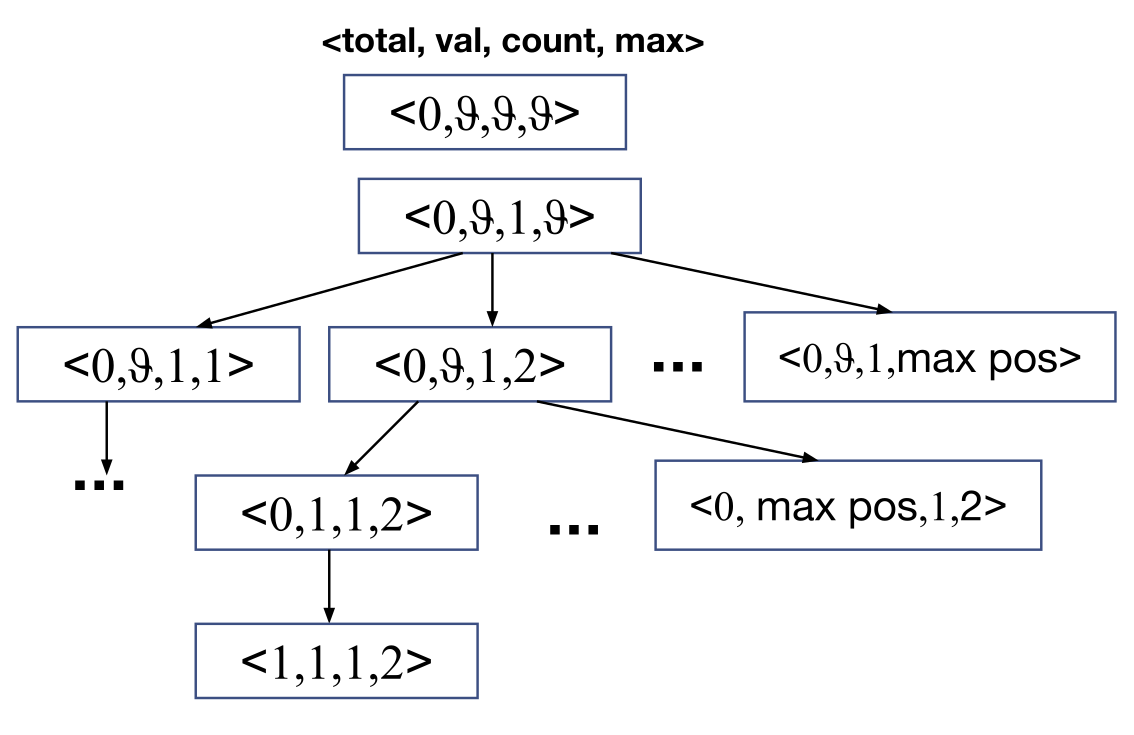
\includegraphics[width=\textwidth]{L05/computation-tree.png}
\end{minipage}
\end{tabular}

The computation tree does indeed represent the space that we want to reason
about. But as a thing that you try to work with, it's unwieldy.
For anything interesting, it's definitely too large to explicitly
create (possibly infinite) or to reason about.

We need abstraction to reason about things. Abstract values, or abstract
flow of control. The abstraction you want to use depends on what you're
trying to establish.

\end{document}
